
\serie{Translation}

\begin{exercice}
Donne les cas où la transformation qui permet de passer de la figure 1 à la figure 2 est une translation :
\begin{center} \includegraphics[width=5.8cm]{translation_figures} \end{center}
\end{exercice}


\begin{exercice}
Quelles sont les cartes images de la carte $T$ par une translation ?
\begin{center} 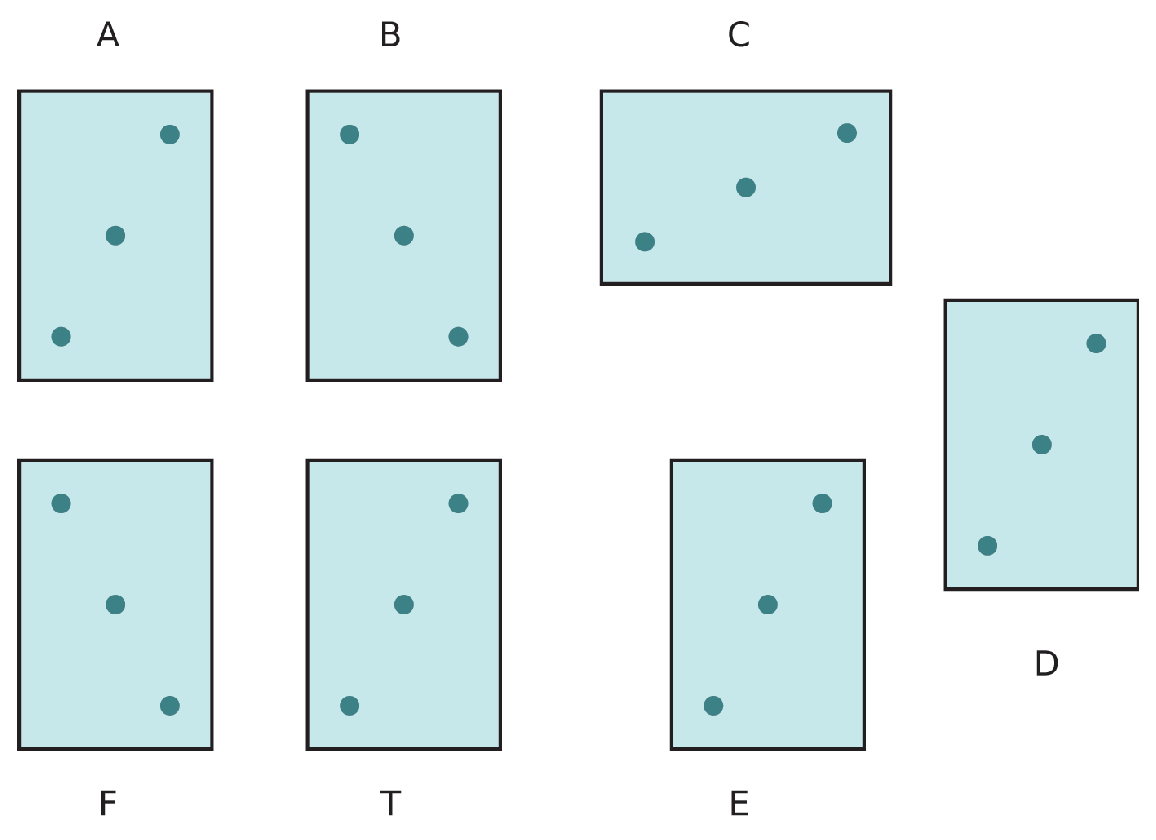
\includegraphics[width=8.1cm]{translation_cartes} \end{center}
\end{exercice}

%%%%%%%%%%%%%%%%%%%%%%%%%%%%%%%%%%%
%%%%%%%%%%%%%%%%%%%%%%%%%%%%%%%%%%%
%MiseEnPage
%%%%%%%%%%%%%%%%%%%%%%%%%%%%%%%%%%%
\columnbreak
%%%%%%%%%%%%%%%%%%%%%%%%%%%%%%%%%%%
%%%%%%%%%%%%%%%%%%%%%%%%%%%%%%%%%%%

\begin{exercice}
Complète les pointillés :
\begin{center} 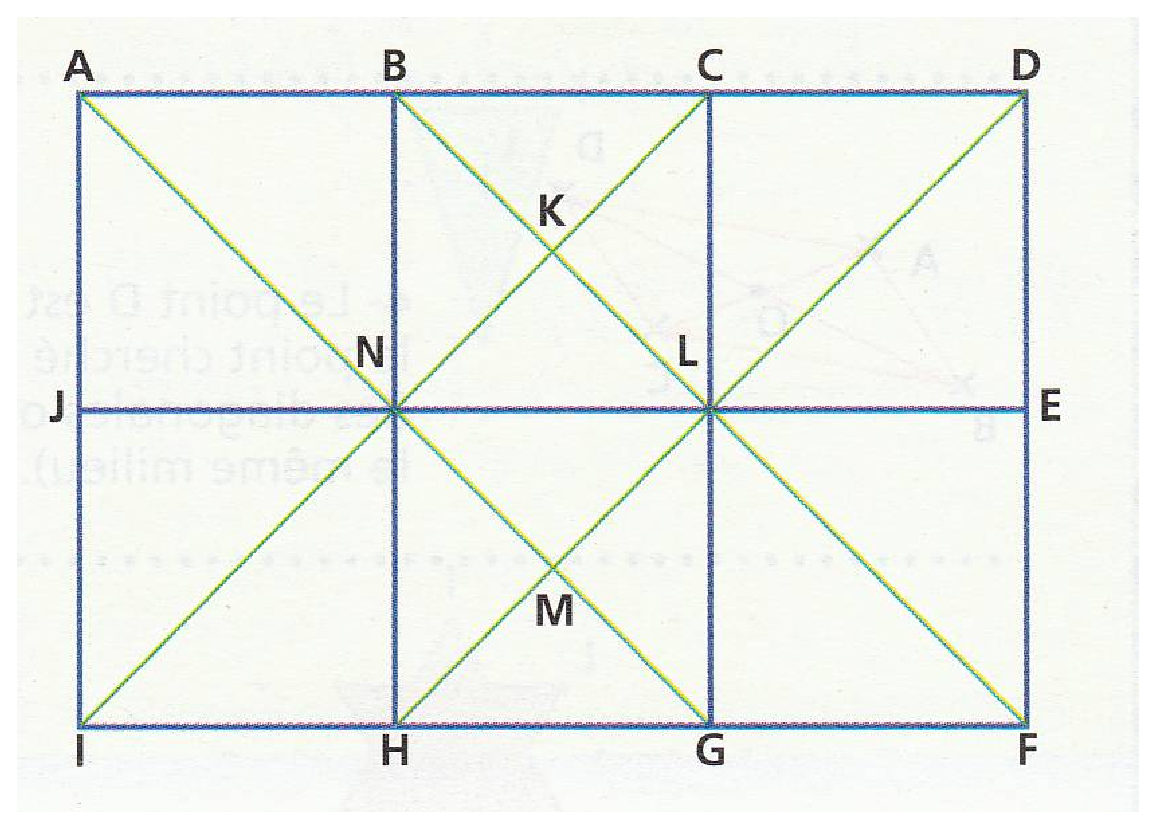
\includegraphics[width=4.5cm]{completer_translation} \end{center}
\begin{enumerate}
 \item L’image du point $L$ par la translation de vecteur $\overrightarrow{AB}$ est \ldots \ldots ;
 \item L’image du point \ldots \ldots par la translation de vecteur $\overrightarrow{BK}$ est $L$ ;
 \item L’image du point $J$ par la translation de vecteur \ldots \ldots est $L$ ;
 \item La translation de vecteur $\overrightarrow{DE}$, transforme $K$ en \ldots \ldots ;
 \item La translation qui transforme \ldots \ldots en $H$, transforme $N$ en $G$ ;
 \item Par la translation de vecteur $\overrightarrow{AJ}$, le triangle $BKN$ a pour image \ldots \ldots ;
 \item Par la translation de vecteur $\overrightarrow{JN}$, le triangle $NLH$ a pour image \ldots \ldots.
 \end{enumerate}
\end{exercice}


\begin{exercice}
Observe la figure ci-après puis recopie et complète dans ton cahier :
\begin{enumerate}
 \item Par la translation de vecteur $\overrightarrow{AC}$, l’image de la figure $\circled{2}$ est la figure \ldots ;
 \item Par la translation de vecteur $\overrightarrow{EC}$, l’image de la figure \ldots est la figure $\circled{2}$ ;
 \item Par la translation qui transforme \ldots en $C$, l’image de la figure $\circled{5}$ est la figure $\circled{6}$ ;
 \item La figure $\circled{3}$ est l’image de la figure \ldots par la translation de vecteur $\overrightarrow{CF}$ ;
 \item Dans la translation qui transforme $E$ en \ldots, l’image de la figure $\circled{3}$ est la figure $\circled{2}$.
 \end{enumerate}
\begin{center} 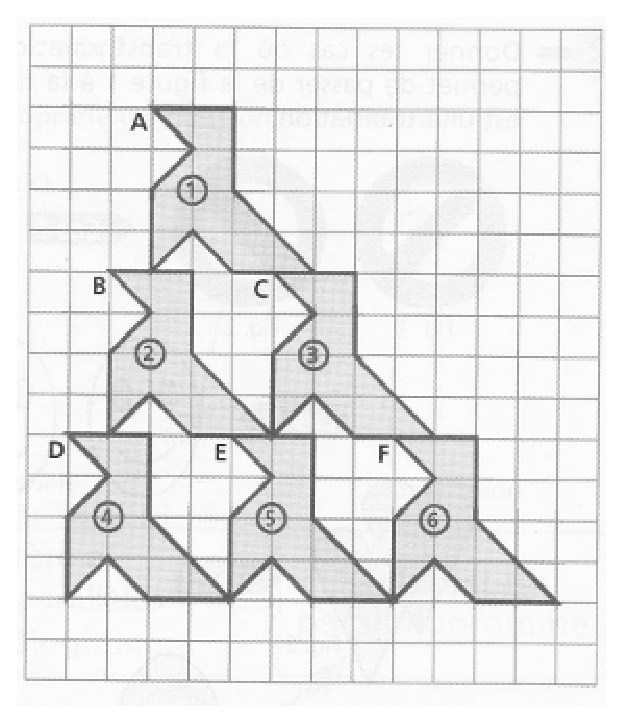
\includegraphics[width=4cm]{pyramide_jaune} \end{center}
\end{exercice}


\begin{exercice}
En t'aidant du quadrillage de ton cahier, recopie puis effectue la translation de vecteur $\vec{b}$ :
\begin{center} 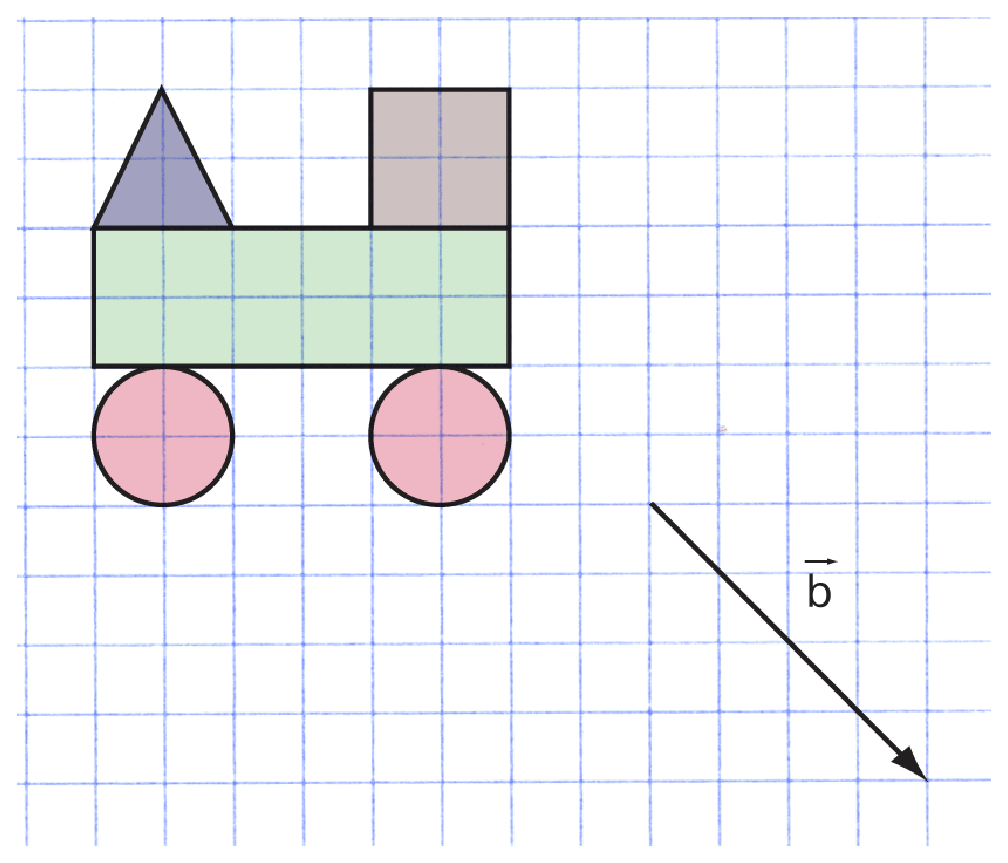
\includegraphics[width=5.4cm]{voiture_vecB} \end{center}
\end{exercice}


\begin{exercice}
En t'aidant du quadrillage de ton cahier, recopie puis effectue les translations :
\begin{center} 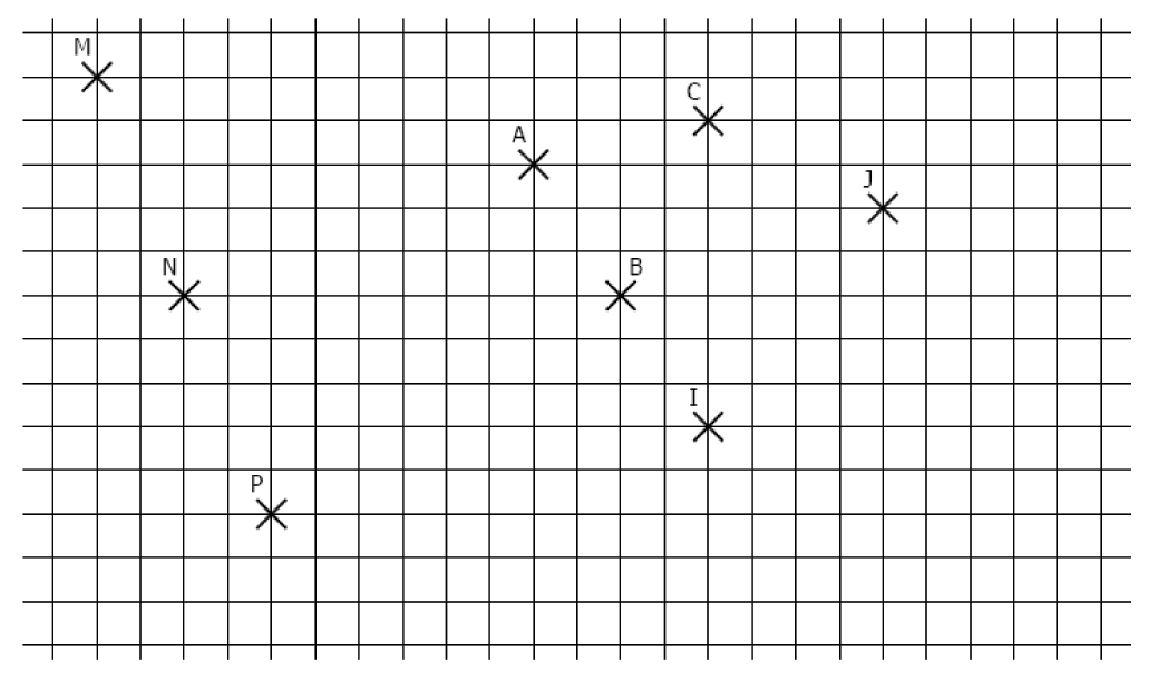
\includegraphics[width=8.1cm]{quadrillage_translations} \end{center}
\begin{enumerate}
 \item Construis le point $M_1$, image de $M$ par la translation de vecteur $\overrightarrow{AB}$ ;
 \item Construis le point $N_1$, image de $N$ par la translation de vecteur $\overrightarrow{AB}$ ;
 \item Construis le point $P_1$, image de $P$ par la translation de vecteur $\overrightarrow{AB}$ ;
 \item Construis le point $M_2$, image de $M$ par la translation de vecteur $\overrightarrow{AC}$ ;
 \item Construis le point $N_2$, image de $N$ par la translation de vecteur $\overrightarrow{AC}$ ;
 \item Construis le point $P_2$, image de $P$ par la translation de vecteur $\overrightarrow{AC}$ ;
 \item Construis le point $I_3$, image de $I$ par la translation de vecteur $\overrightarrow{MN}$ ;
 \item Construis le point $J_3$, image de $J$ par la translation de vecteur $\overrightarrow{MN}$ ;
 \item Construis le point $A_4$, image de $A$ par la translation de vecteur $\overrightarrow{BA}$ ;
 \item Construis le point $B_4$, image de $B$ par la translation de vecteur $\overrightarrow{BA}$.
 \end{enumerate}
\end{exercice}


\begin{exercice}
$[CD]$ est-il l'image de $[AB]$ par une translation ? Justifie ta réponse.
\begin{center} 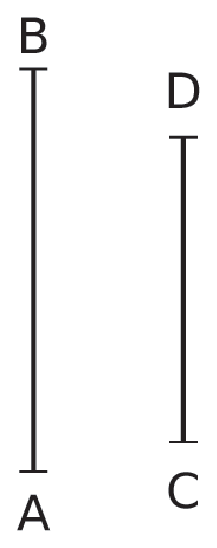
\includegraphics[width=1.2cm]{imageAB_CD} \end{center}
\end{exercice}


\begin{exercice}[Dans un repère]
Dans ton cahier trace un repère d'unité 1 cm pour chaque axe, puis place les points suivants : \\[0.5em]
\begin{tabular}{l|l}
$A(+ 3 ; + 2)$ \phantom{HELLO} & $D(+ 1 ; - 3)$ \\
$B(- 4 ; + 3)$ \phantom{HELLO} & $O(0 ; 0)$ \\
$C(- 2 ; - 1)$ \phantom{HELLO} & $T(+ 2 ; - 3)$ \\
 \end{tabular} \\

On considère la translation de vecteur $\overrightarrow{OT}$. Quelles sont les coordonnées des points $A'$, $B'$, $C'$, $D'$, images des points $A$, $B$, $C$, $D$ par cette translation.
\end{exercice}

%%%%%%%%%%%%%%%%%%%%%%%%%%%%%%%%%%%%%%%%%%%%%%%%%%%%%%%%%%%%%%%%%%%%%%%%%

\serie{Rotation}

\begin{exercice}
Détermine sur la figure ci-dessous quelles sont les images des points donnés par la rotation indiquée :
\begin{colenumerate}{2}
 \item $G$ par $R(O ; + 30^\circ)$ ;
 \item $T$ par $R(O ; + 60^\circ)$ ;
 \item $M$ par $R(O ; - 30^\circ)$ ;
 \item $I$ par $R(O ; - 60^\circ)$ ;
 \item $F$ par $R(O ; + 90^\circ)$ ;
 \item $G$ par $R(O ; - 120^\circ)$ ;
 \item $E$ par $R(O; + 120^\circ)$ ;
 \item $O$ par $R(O ; + 60^\circ)$ ;
 \item $E$ par $R(O ; + 180^\circ)$.
 \end{colenumerate}
\begin{center} 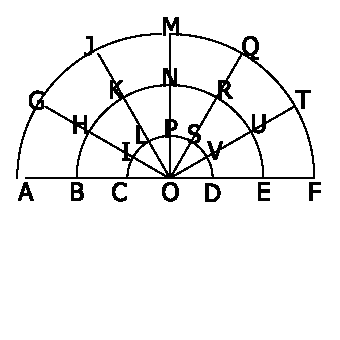
\includegraphics[width=5.6cm]{lettres_rotation} \end{center}
\end{exercice}

%%%%%%%%%%%%%%%%%%%%%%%%%%%%%%%%%%%
%%%%%%%%%%%%%%%%%%%%%%%%%%%%%%%%%%%
%MiseEnPage
%%%%%%%%%%%%%%%%%%%%%%%%%%%%%%%%%%%
\newpage
%%%%%%%%%%%%%%%%%%%%%%%%%%%%%%%%%%%
%%%%%%%%%%%%%%%%%%%%%%%%%%%%%%%%%%%

\vspace{-2.5cm}
\begin{exercice}
Détermine sur la figure ci-dessous, l'angle de la rotation de centre $O$ telle que l'image de \ldots
\begin{colenumerate}{3}
 \item $M$ donne $J$ ;
 \item $U$ donne $N$ ;
 \item $K$ donne $N$ ;
 \item $P$ donne $V$ ;
 \item $D$ donne $I$ ;
 \item $H$ donne $U$ ;
 \item $B$ donne $U$ ;
 \item $F$ donne $A$ ;
 \item $I$ donne $S$.
 \end{colenumerate}
\begin{center} 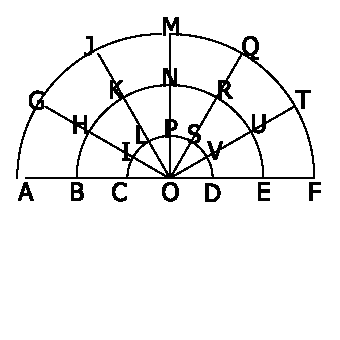
\includegraphics[width=5.6cm]{lettres_rotation} \end{center}
\end{exercice}


\vspace{-2.5cm}
\begin{exercice}
En t'aidant du quadrillage de ton cahier reporte les points suivants :
\begin{center} 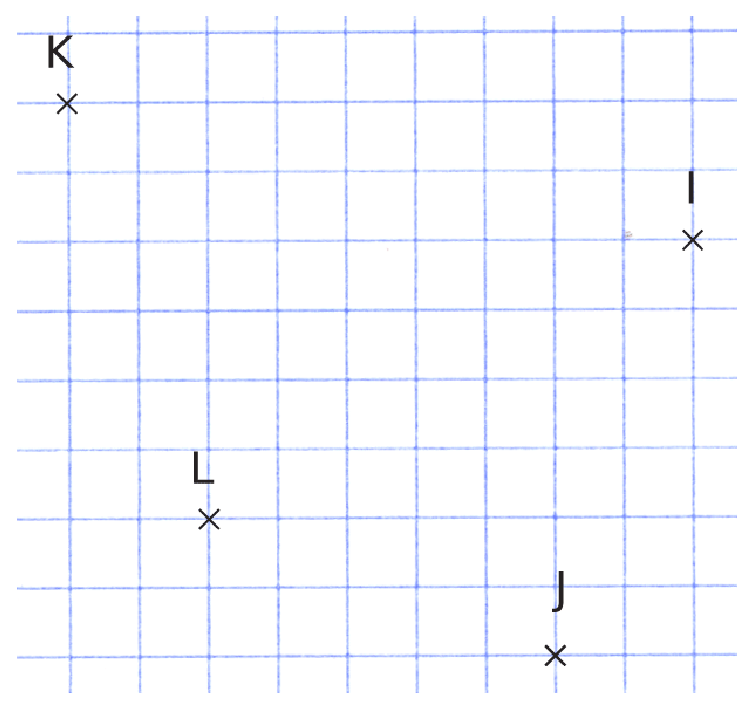
\includegraphics[width=5.4cm]{quadrillageKLJI} \end{center}
Construis le point :
\begin{enumerate}
 \item $J_1$ image de $J$ par la rotation de centre $I$ et d’angle $+ 90^\circ$ ;
 \item $K_1$ image de $K$ par la rotation de centre $I$ et d’angle $- 90^\circ$ ;
 \item $L_1$ image de $L$ par la rotation de centre $I$ et d’angle $+ 90^\circ$ ;
 \item $I_2$ image de $I$ par la rotation de centre $K$ et d’angle $- 45^\circ$ ;
 \item $J_2$ image de $J$ par la rotation de centre $K$ et d’angle $+ 45^\circ$ ;
 \item $L_2$ image de $L$ par la rotation de centre $K$ et d’angle $- 45^\circ$.
 \end{enumerate}
\end{exercice}


\begin{exercice}
Reproduis la lettre $F$ dans ton cahier. Construis l'image la lettre $F$ par la rotation de centre $O$, d'angle $+ 90^\circ$.
\begin{center} 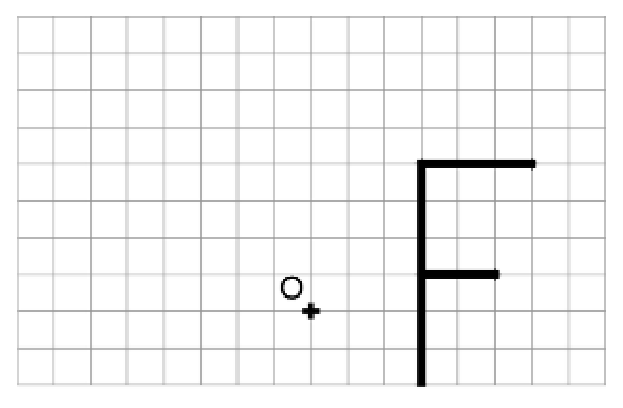
\includegraphics[width=8.1cm]{quadrillageF} \end{center}
\end{exercice}


\begin{exercice}
Reproduis la lettre $E$ dans ton cahier. Construis l'image de lettre $E$ par la rotation de centre $O$, d'angle $- 45^\circ$.
\begin{center} 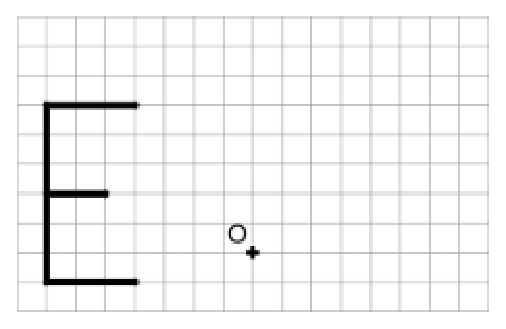
\includegraphics[width=8.1cm]{quadrillageE} \end{center}
\end{exercice}


\begin{exercice}
Soit $ABC$ un triangle tel que $\widehat{BAC}$ mesure $60^\circ$; $[AB]$ mesure 4cm et $[AC]$ mesure 3cm. Soit $O$ un point extérieur au triangle $ABC$.
\begin{enumerate}
 \item Faire une figure sur une feuille blanche ;
 \item Construire le triangle $A'B'C'$ image du triangle $ABC$ par la rotation de centre $O$, d'angle $+ 40^\circ$.
 \end{enumerate}
\end{exercice}


\begin{exercice}
Soit $A$ et $B$ deux point distincts. Soit $E$ l'image de $B$ par la rotation de centre $A$, d'angle $+ 30^\circ$. Soit $F$ l'image de $B$ par la rotation de centre $A$, d'angle $- 60^\circ$.
\begin{enumerate}
 \item Trace la figure.
 \item Quelle est la nature du triangle $AEF$ ?
 \end{enumerate}
\end{exercice}
